\documentclass[11pt]{article}
\usepackage[margin=1in]{geometry}
\usepackage{amsmath,amssymb,amsthm,mathtools}
\usepackage{booktabs,tabularx,array,longtable}
\usepackage{xcolor}
\usepackage{enumitem}
\usepackage{hyperref}
\usepackage{microtype}
\usepackage{tikz}
\usepackage{tikz-cd}
\usepackage{fancyhdr}
\usepackage{titlesec}
\usepackage{newtxtext,newtxmath}
\usetikzlibrary{positioning,arrows.meta,calc}

\definecolor{navy}{RGB}{35,55,85}
\definecolor{softblue}{RGB}{235,242,250}
\definecolor{softgray}{RGB}{246,246,246}
\definecolor{softgreen}{RGB}{237,247,240}
\definecolor{softgold}{RGB}{251,246,232}
\hypersetup{colorlinks=true,linkcolor=navy,citecolor=navy,urlcolor=navy}
\titleformat{\section}{\Large\bfseries\color{navy}}{\thesection}{0.7em}{}
\titleformat{\subsection}{\large\bfseries\color{navy}}{\thesubsection}{0.7em}{}
\pagestyle{fancy}
\setlength{\headheight}{14pt}
\fancyhf{}
\lhead{ProLT Homotopy-Preserving Observations}
\rhead{Working note v0.4}
\cfoot{\thepage}
\setlength{\parindent}{0pt}
\setlength{\parskip}{0.55em}

\newtheorem{theorem}{Theorem}[section]
\newtheorem{proposition}[theorem]{Proposition}
\newtheorem{lemma}[theorem]{Lemma}
\newtheorem{corollary}[theorem]{Corollary}
\theoremstyle{definition}
\newtheorem{definition}[theorem]{Definition}
\newtheorem{example}[theorem]{Example}
\newtheorem{remark}[theorem]{Remark}

\newcommand{\F}{\mathbb F_2}
\newcommand{\Om}{\Omega_P}
\newcommand{\truth}{\varsigma}
\newcommand{\OX}{\mathcal O}
\newcommand{\K}{\mathcal K}
\newcommand{\im}{\operatorname{im}}
\newcommand{\rank}{\operatorname{rank}}
\newcommand{\xor}{\mathbin{\Updownarrow}}
\newcommand{\sd}{\operatorname{sd}}
\newcommand{\Mod}{\operatorname{Mod}}
\newcommand{\statusS}{\textbf{[S]}}
\newcommand{\statusA}{\textbf{[A]}}
\newcommand{\statusC}{\textbf{[C]}}

\begin{document}

\begin{center}
{\LARGE\bfseries\color{navy} Homotopy-Preserving Logical Observations in Propositional Logical Topologies}\par
\vspace{0.35em}
{\large Repair maps, closure systems, Horn-type criteria, and the height-two repair-forest theorem}\par
\vspace{0.7em}
{\normalsize Working research note v0.4 --- 23 September 2026}\par
\vspace{0.3em}
{\small Continuation of \emph{Homological Foundations for Propositional Logical Topologies} (v0.1), \emph{Observation Refinement Classification} (v0.2), and \emph{Controlled Refinement Regimes} (v0.3).}
\end{center}

\vspace{0.8em}
\noindent\colorbox{softgold}{\parbox{0.96\textwidth}{
\textbf{Status convention.} \statusS\ denotes standard mathematics used essentially unchanged; \statusA\ denotes a direct ProLT specialization or elementary derived result; \statusC\ denotes a contribution candidate whose novelty is not claimed before a dedicated adversarial literature audit. The strongest new candidate in this note is the exact height-two \emph{repair-forest theorem}, which converts one-bit post-$T_0$ refinement into a rooted graph and makes homotopy preservation equivalent to a tree/forest condition.
}}

\section{Purpose and relation to the previous stages}

The ProLT core manuscript starts with an indexed observation family $\Phi$, its signature map $o_\Phi$, and the finite topology generated by positive truth regions. Its key order-theoretic fact is
\[
p\preceq_\Phi q
\quad\Longleftrightarrow\quad
o_\Phi(p)\subseteq o_\Phi(q).
\]
The v0.1 note then defined canonical ProLT homology using the order complex of the realized-signature poset. The v0.2 note classified arbitrary refinements through their new-coordinate fiber profiles and introduced mapping-cone defect homology. The v0.3 note specialized to post-$T_0$ refinement, where no state splitting remains: refinement keeps the same vertices and only deletes old order comparisons. It proved, among other results:
\begin{enumerate}[label=(\roman*)]
\item positive/isotone added observations are exactly the topologically redundant one-bit observations;
\item nonconstant antitone added observations split connected components and change $H_0$;
\item height at most one is rigid: every nonredundant post-$T_0$ refinement changes homology;
\item height two admits an exact relative-boundary-matrix test;
\item over a coarse chain, one added bit is homotopy-defective exactly for a nonconstant nonincreasing threshold word.
\end{enumerate}

The present goal is more operational:
\begin{quote}
\emph{Which logically recognizable kinds of new observations are guaranteed to preserve the homotopy type of the canonical ProLT order complex?}
\end{quote}

Two answers are developed. First, in arbitrary height, we obtain constructive \emph{repair-map} criteria, with closure-system and Horn-type corollaries. Second, in height two, the previous relative matrix becomes a graph incidence matrix, producing an exact rooted-forest characterization and an explicit greedy collapse algorithm.

\section{Post-$T_0$ one-bit refinement}

Assume throughout this section that the coarse ProLT is already $T_0$. Write
\[
P:=P_\Phi
\]
for its realized-signature poset. Let $\psi$ be one new observation and define
\[
b(p):=1[p\models\psi]\in\{0,1\}.
\]
The refined poset has the same underlying set and order
\begin{equation}\label{eq:fineorder}
p\le_b q
\quad\Longleftrightarrow\quad
p\le q\text{ in }P
\quad\text{and}\quad
b(p)\le b(q).
\end{equation}
Write
\[
Q_b:=(P,\le_b),\qquad
K:=\Delta(P),\qquad
L_b:=\Delta(Q_b)\subseteq K.
\]

\begin{definition}[Descent]
A comparable pair $p<q$ is a \emph{$b$-descent} when
\[
b(p)=1,
\qquad
b(q)=0.
\]
Equivalently, $[p,q]$ is an edge of $K$ deleted by the refinement.
\end{definition}

\begin{proposition}[Deleted-chain criterion]\label{prop:deletedchain}
\statusA\;
A coarse chain
\[
p_0<p_1<\cdots<p_k
\]
survives as a simplex of $L_b$ if and only if
\[
b(p_0)\le b(p_1)\le\cdots\le b(p_k).
\]
Thus a simplex is deleted exactly when its Boolean word contains a $1\to0$ descent.
\end{proposition}

This makes the logical content of refinement very concrete: after $T_0$, a new Boolean observation deletes precisely those information chains along which the new truth value reverses from true to false.

\section{Repair maps: arbitrary-height sufficient criteria}

The simplest way to prove that $L_b\hookrightarrow K$ is a homotopy equivalence is to construct a monotone map that systematically moves every old state to a ``safe'' state without leaving its old information direction.

\subsection{General repair-map theorem}

\begin{theorem}[Down-repair criterion]\label{thm:downrepair}
\statusS/\statusA/\statusC\;
Suppose there exists an order-preserving map
\[
\rho:P\longrightarrow P
\]
such that, for every $p\in P$,
\begin{equation}\label{eq:downrepair}
\rho(p)\le p,
\qquad
b(\rho(p))=0.
\end{equation}
Then the inclusion
\[
i:Q_b\hookrightarrow P
\]
induces a homotopy equivalence
\[
\Delta(Q_b)\simeq\Delta(P).
\]
The map $\rho$, regarded as a map $P\to Q_b$, is a homotopy inverse.
\end{theorem}

\begin{proof}
Because $\rho$ is monotone in $P$ and every value of $b\circ\rho$ is $0$, the map $\rho:P\to Q_b$ is monotone. Moreover,
\[
i\rho(p)=\rho(p)\le p
\]
in $P$. For $p\in Q_b$, condition \eqref{eq:downrepair} also gives
\[
\rho(p)\le_b p,
\]
because $0=b(\rho(p))\le b(p)$. Hence
\[
i\rho\le\operatorname{id}_P,
\qquad
\rho i\le\operatorname{id}_{Q_b}.
\]
Pointwise comparable monotone maps induce homotopic maps on order complexes, so $\Delta(i)$ and $\Delta(\rho)$ are homotopy inverses.
\end{proof}

\begin{theorem}[Up-repair criterion]\label{thm:uprepair}
\statusS/\statusA/\statusC\;
Dually, suppose there exists an order-preserving map
\[
\lambda:P\longrightarrow P
\]
such that
\[
p\le\lambda(p),
\qquad
b(\lambda(p))=1
\]
for every $p$. Then $L_b\hookrightarrow K$ is a homotopy equivalence, with $\lambda:P\to Q_b$ as a homotopy inverse.
\end{theorem}

\begin{remark}[Interpretation]
A down-repair monotonically weakens every information state to a $\psi$-false state. An up-repair monotonically strengthens every state to a $\psi$-true state. Either construction routes every state through a region on which the new observation has constant truth value, so the newly forbidden true-to-false comparisons can be bypassed without changing homotopy type.
\end{remark}

\subsection{Canonical false floors and true ceilings}

Let
\[
F_\psi:=\{p:b(p)=0\},
\qquad
T_\psi:=\{p:b(p)=1\}.
\]

\begin{definition}[False-floor property]
The observation $\psi$ has the \emph{false-floor property} when, for every $p\in P$, the set
\[
F_\psi\cap\downarrow p
\]
has a greatest element, denoted $\lfloor p\rfloor_F$.
\end{definition}

\begin{definition}[True-ceiling property]
The observation $\psi$ has the \emph{true-ceiling property} when, for every $p\in P$, the set
\[
T_\psi\cap\uparrow p
\]
has a least element, denoted $\lceil p\rceil_T$.
\end{definition}

\begin{theorem}[Floor/ceiling preservation]\label{thm:floorceil}
\statusS/\statusA/\statusC\;
If $\psi$ has either the false-floor property or the true-ceiling property, then adding $\psi$ preserves the homotopy type of the canonical ProLT order complex.
\end{theorem}

\begin{proof}
For the false-floor case define
\[
\rho(p)=\lfloor p\rfloor_F.
\]
If $p\le q$, then every false state below $p$ is also below $q$, so maximality gives
\[
\rho(p)\le\rho(q).
\]
Thus $\rho$ is monotone, lies below the identity, and takes only false values. Apply Theorem~\ref{thm:downrepair}. The true-ceiling case is dual.
\end{proof}

\begin{remark}[Closure-operator form]
The floor map is an interior operator: it is monotone, idempotent, and satisfies $\rho(p)\le p$. The ceiling map is a closure operator: it is monotone, idempotent, and satisfies $p\le\lambda(p)$. Closure/interior operators are standard homotopy tools in finite-poset topology; the ProLT content here is the interpretation of their fixed-point regions as truth-value repair regions for a new observation.
\end{remark}

\subsection{Extremal anchors}

\begin{corollary}[Componentwise cone-anchor criterion]\label{cor:anchor}
\statusA/\statusC\;
Suppose every connected component $C$ of $P$ satisfies at least one of the following:
\begin{enumerate}[label=(\roman*)]
\item $C$ has a least element $\bot_C$ with $b(\bot_C)=0$;
\item $C$ has a greatest element $\top_C$ with $b(\top_C)=1$.
\end{enumerate}
Then refinement by $\psi$ preserves homotopy type.
\end{corollary}

\begin{proof}
In case (i), the constant map $p\mapsto\bot_C$ on that component is a down-repair. In case (ii), the constant map $p\mapsto\top_C$ is an up-repair. The componentwise maps combine because distinct components have no comparisons.
\end{proof}

\begin{corollary}[Endpoint test on a Boolean-lattice signature space]\label{cor:endpoint}
If
\[
P=2^I
\]
with its usual inclusion order, then adding one observation $\psi$ is guaranteed to preserve homotopy whenever
\[
b(\varnothing)=0
\quad\text{or}\quad
b(I)=1.
\]
Consequently, only the endpoint-reversing case
\[
b(\varnothing)=1,
\qquad
b(I)=0
\]
can possibly change homotopy type.
\end{corollary}

\begin{remark}
This criterion is intentionally only about the canonical order-complex homotopy type. A nonredundant observation satisfying the endpoint test can still delete many order relations, alter specialization structure, and change signature distances.
\end{remark}

\section{Semilattice and Horn-type observation classes}

The floor/ceiling criterion has a useful algebraic form when the realized-signature poset has meet or join structure.

\begin{theorem}[Join-closed falsity gives a down-repair]\label{thm:joinfalse}
\statusS/\statusA/\statusC\;
Assume $P$ is a finite join-semilattice. Suppose:
\begin{enumerate}[label=(\roman*)]
\item $F_\psi$ is closed under finite joins in $P$; and
\item $F_\psi\cap\downarrow p\ne\varnothing$ for every $p\in P$.
\end{enumerate}
Then $\psi$ has the false-floor property, with
\[
\lfloor p\rfloor_F
=
\bigvee(F_\psi\cap\downarrow p),
\]
and therefore preserves homotopy type.
\end{theorem}

\begin{proof}
The displayed join lies in $F_\psi$ by join closure. Since $p$ is an upper bound for every element being joined, the join is still at most $p$. It is clearly above every false element below $p$, hence is the required greatest false predecessor.
\end{proof}

\begin{theorem}[Meet-closed truth gives an up-repair]\label{thm:meettrue}
\statusS/\statusA/\statusC\;
Assume $P$ is a finite meet-semilattice. Suppose:
\begin{enumerate}[label=(\roman*)]
\item $T_\psi$ is closed under finite meets in $P$; and
\item $T_\psi\cap\uparrow p\ne\varnothing$ for every $p\in P$.
\end{enumerate}
Then $\psi$ has the true-ceiling property, with
\[
\lceil p\rceil_T
=
\bigwedge(T_\psi\cap\uparrow p),
\]
and therefore preserves homotopy type.
\end{theorem}

\begin{corollary}[Horn-type repair]\label{cor:horn}
Suppose the realized-signature poset is a meet-subsemilattice of a Boolean cube, and the truth states of $\psi$ are the models of a Horn CNF in the old observation coordinates. If every realized signature lies below at least one such model, then $\psi$ preserves homotopy type.
\end{corollary}

\begin{proof}
Model sets of Horn CNF theories are closed under coordinatewise intersection, i.e. meet. The result is Theorem~\ref{thm:meettrue}.
\end{proof}

\begin{corollary}[Dual-Horn falsity repair]
Dually, suppose $P$ is a join-subsemilattice and the $\psi$-false signatures form a union-closed (equivalently, in the usual Boolean-relation setting, dual-Horn definable) family which is lower cofinal. Then $\psi$ preserves homotopy type.
\end{corollary}

\begin{remark}[Why the Horn statement is not a novelty claim]
Horn formulas, closure systems, and their induced closure operators are classical and highly developed. The point here is not that Horn models form closure systems; it is that those closure operators become explicit homotopy-inverse certificates for ProLT observation refinement under the stated cofinality hypotheses.
\end{remark}

\section{Height two: from a boundary matrix to a repair forest}

We now obtain an exact answer in the first dimension where nonredundant homotopy-neutral refinement is possible.

Assume
\[
\operatorname{ht}(P)\le2.
\]
Let
\[
E_{\rm del}
\]
be the set of deleted edges, equivalently the $b$-descents, and let
\[
T_{\rm del}
\]
be the set of deleted triangles. The v0.3 height-two theorem gives the relative chain complex
\[
0\longrightarrow
\F[T_{\rm del}]
\overset{\partial_2^{\rm rel}}{\longrightarrow}
\F[E_{\rm del}]
\longrightarrow0.
\]

\subsection{The four deleted Boolean triangle patterns}

For a coarse chain
\[
x<y<z,
\]
the surviving bit words are
\[
000,\quad001,\quad011,\quad111.
\]
The four deleted words are:

\begin{center}
\begin{tabular}{ccl}
\toprule
word & number of deleted edges & deleted edges \\
\midrule
$010$ & $1$ & $[y,z]$ \\
$101$ & $1$ & $[x,y]$ \\
$100$ & $2$ & $[x,y],\,[x,z]$ \\
$110$ & $2$ & $[x,z],\,[y,z]$ \\
\bottomrule
\end{tabular}
\end{center}

Thus every column of $\partial_2^{\rm rel}$ has Hamming weight either one or two. That special binary fact is what turns the relative boundary matrix into an ordinary graph incidence matrix.

\subsection{Definition of the repair graph}

\begin{definition}[Rooted repair graph]\label{def:repairgraph}
For each connected component $C$ of the coarse poset $P$, introduce one formal root vertex $*_C$. Introduce one additional graph vertex $v_e$ for every deleted edge $e\in E_{\rm del}$. For every deleted triangle $\tau\in T_{\rm del}$:
\begin{enumerate}[label=(\roman*)]
\item if $\tau$ contains exactly one deleted edge $e$, add a graph edge joining $*_C$ to $v_e$, where $C$ is the coarse component containing $\tau$;
\item if $\tau$ contains exactly two deleted edges $e,f$, add a graph edge joining $v_e$ to $v_f$.
\end{enumerate}
The resulting (possibly multi-)graph is denoted
\[
\mathfrak R_\psi(P).
\]
\end{definition}

The one-descent triangles $010$ and $101$ are therefore \emph{anchors}: they attach a descent edge directly to the component root. The two-descent triangles $100$ and $110$ express a dependency between two descent edges.

\begin{proposition}[Relative boundary as reduced incidence]\label{prop:incidence}
\statusS/\statusA/\statusC\;
Over $\F$, the relative boundary matrix
\[
\partial_2^{\rm rel}
\]
is exactly the vertex-edge incidence matrix of $\mathfrak R_\psi(P)$ after deleting the rows corresponding to the formal roots.
\end{proposition}

\begin{proof}
A $010$ or $101$ triangle has one deleted edge, so its relative boundary column has one $1$; the corresponding repair-graph edge joins that deleted-edge vertex to a root, whose incidence row is subsequently removed. A $100$ or $110$ triangle has two deleted edges, so its relative boundary column has two $1$s; the corresponding graph edge joins the two deleted-edge vertices. These are all possible deleted bit patterns.
\end{proof}

\subsection{Exact repair-forest theorem}

\begin{theorem}[Height-two repair-forest theorem]\label{thm:repairforest}
\statusS/\statusA/\statusC\;
Assume $P$ is post-$T_0$ and $\operatorname{ht}(P)\le2$. For one added observation $\psi$, the following are equivalent:
\begin{enumerate}[label=(\roman*)]
\item the inclusion $L_b\hookrightarrow K$ is a homotopy equivalence;
\item it is a simple homotopy equivalence;
\item $K$ simplicially collapses onto $L_b$ using only deleted edge--triangle pairs;
\item it is a homology equivalence over $\F$;
\item $\partial_2^{\rm rel}$ is invertible;
\item the rooted repair graph $\mathfrak R_\psi(P)$ is a forest in which every connected component contains exactly one formal root.
\end{enumerate}
Thus, in height two for one new observation,
\[
\boxed{\text{homology-neutral}\iff\text{homotopy-neutral}\iff\text{repair forest}.}
\]
\end{theorem}

\begin{proof}
The implications (iii)$\Rightarrow$(ii)$\Rightarrow$(i)$\Rightarrow$(iv) are standard. The v0.3 height-two relative-chain theorem gives (iv)$\Leftrightarrow$(v).

By Proposition~\ref{prop:incidence}, the matrix in (v) is a reduced incidence matrix of $\mathfrak R_\psi(P)$. Suppose it is invertible. Then the number of graph edges equals the number of nonroot vertices. A cycle would give a nontrivial mod-$2$ linear dependence among its incidence columns. A connected component containing no root would give a row dependence by summing all nonroot incidence rows in that component. A component containing two roots would give a column dependence along the unique path between those roots after the root rows are deleted. Hence the graph is acyclic and every component contains exactly one root, proving (v)$\Rightarrow$(vi).

Conversely, suppose (vi) holds. Each rooted tree with at least one nonroot vertex has a nonroot leaf. That leaf corresponds to a deleted edge $e$ contained in exactly one remaining deleted triangle $\tau$. A retained triangle cannot contain a deleted edge because $L_b$ is a subcomplex; there are no cells above dimension two. Hence $e$ is a free face of $\tau$, so $(e,\tau)$ is an elementary collapse pair. Removing it prunes one nonroot leaf and its incident repair-graph edge, leaving another rooted forest. Iterating removes all deleted cells and leaves exactly $L_b$. Thus (vi)$\Rightarrow$(iii), closing the cycle of equivalences.
\end{proof}

\begin{corollary}[Greedy logical collapse algorithm]\label{cor:greedy}
At height two, the following algorithm decides whether one added observation preserves homotopy:
\begin{enumerate}[label=\arabic*.]
\item list every descent edge $p<q$ with $b(p)=1,b(q)=0$;
\item list every deleted three-chain $x<y<z$;
\item repeatedly choose a currently deleted edge contained in exactly one currently deleted triangle and remove that edge--triangle pair;
\item succeed if all deleted cells are exhausted; fail otherwise.
\end{enumerate}
The algorithm succeeds if and only if the refinement preserves homotopy.
\end{corollary}

\begin{proof}
The algorithm is exactly nonroot-leaf pruning in the repair graph. It exhausts the graph precisely when every component is a rooted tree.
\end{proof}

\begin{corollary}[Local repair interpretation]
A one-bit height-two refinement preserves homotopy exactly when every cluster of descent edges has:
\begin{enumerate}[label=(\roman*)]
\item a path of two-descent repair dependencies leading to a one-descent anchor triangle; and
\item no cyclic repair dependency.
\end{enumerate}
Equivalently, every descent cluster has exactly one root anchor in the repair forest.
\end{corollary}

\begin{remark}[Why this is stronger than the v0.3 matrix test]
The v0.3 criterion required constructing $\partial_2^{\rm rel}$ and checking invertibility. The repair-forest theorem replaces Gaussian elimination by a purely combinatorial condition and simultaneously upgrades an exact homology test to an exact homotopy and collapse test.
\end{remark}

\section{Worked Boolean example: $\Phi=(X,Y)$}

Let
\[
D=\varnothing,
\quad
A=\{X\},
\quad
C=\{Y\},
\quad
B=\{X,Y\}.
\]
Then
\[
D<A<B,
\qquad
D<C<B,
\]
so $P_\Phi$ is the Boolean diamond $B_2$. Its order complex is two filled triangles $DAB$ and $DCB$ glued along $DB$.

\subsection{Positive observation: $X\vee Y$}

The bit profile is
\[
0,1,1,1
\]
on $(D,A,C,B)$. It is isotone, so the observation is topologically redundant. No edge or simplex is deleted.

\subsection{XOR: nonredundant but homotopy-preserving}

For
\[
\psi=X\xor Y,
\]
the profile is
\[
0,1,1,0.
\]
The deleted edges are
\[
A<B,
\qquad
C<B.
\]
The deleted triangles have words $010$ and $010$, so each has exactly one deleted edge. The repair graph is
\[
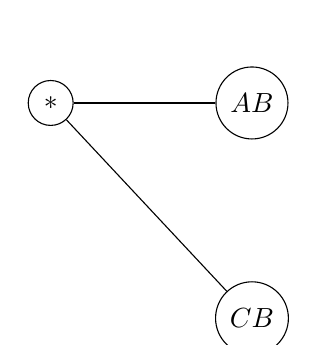
\begin{tikzpicture}[baseline=-0.6ex,node distance=1.8cm]
\node[circle,draw] (r) {$*$};
\node[circle,draw,right=of r] (e1) {$AB$};
\node[circle,draw,below=of e1] (e2) {$CB$};
\draw[-] (r)--(e1);
\draw[-] (r)--(e2);
\end{tikzpicture}
\]
a rooted tree. Hence
\[
\OX_{(X,Y,X\xor Y)}\simeq\OX_{(X,Y)}.
\]
The refinement is nevertheless nonredundant: it deletes specialization relations and changes the topology.

\subsection{XNOR: another nonredundant neutral observation}

For
\[
\psi=X\Leftrightarrow Y,
\]
the profile is
\[
1,0,0,1.
\]
The deleted edges are $D<A$ and $D<C$. Each deleted triangle has word $101$, again producing a rooted two-leaf tree. Homotopy type is preserved. The global maximum $B$ is also a true cone anchor, so Corollary~\ref{cor:anchor} supplies an independent certificate.

\subsection{NOR: guaranteed homotopy change}

For
\[
\psi=\neg(X\vee Y),
\]
the profile is
\[
1,0,0,0.
\]
This is nonconstant antitone. The deleted edges are
\[
D<A,
\quad
D<C,
\quad
D<B.
\]
The two deleted triangles both have word $100$. The repair graph has an isolated root and an unrooted tree on the three descent-edge vertices:
\[
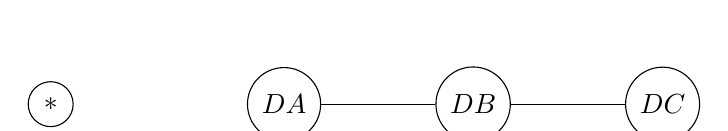
\begin{tikzpicture}[baseline=-0.6ex,node distance=1.45cm]
\node[circle,draw] (r) {$*$};
\node[circle,draw,right=2.2cm of r] (e1) {$DA$};
\node[circle,draw,right=of e1] (e2) {$DB$};
\node[circle,draw,right=of e2] (e3) {$DC$};
\draw[-] (e1)--(e2);
\draw[-] (e2)--(e3);
\end{tikzpicture}
\]
so the rooted-forest criterion fails. Indeed the refined poset separates $D$ from the remaining component, changing $H_0$.

\section{A taxonomy of logically recognizable guarantees}

The results now give several increasingly broad families of homotopy-preserving observations.

\begin{longtable}{>{\raggedright\arraybackslash}p{0.27\textwidth}>{\raggedright\arraybackslash}p{0.27\textwidth}>{\raggedright\arraybackslash}p{0.38\textwidth}}
\toprule
Observation class / condition & Guarantee & Mechanism \\
\midrule
\endfirsthead
\toprule
Observation class / condition & Guarantee & Mechanism \\
\midrule
\endhead
$b$ isotone on $P_\Phi$ & Topology unchanged & No descent edge exists; the observation is already open/redundant. \\
Down-repair exists & Homotopy preserved & Monotone weakening into a constant-false repair region. \\
Up-repair exists & Homotopy preserved & Monotone strengthening into a constant-true repair region. \\
False-floor or true-ceiling property & Homotopy preserved & Canonical interior/closure operator. \\
Least state false or greatest state true in each component & Homotopy preserved & Each refined component remains a cone. \\
Meet-closed, upper-cofinal truth set & Homotopy preserved & Closure operator; includes Horn-type cases on meet-semilattice signatures. \\
Join-closed, lower-cofinal false set & Homotopy preserved & Interior operator; dual closure-system criterion. \\
One bit over a coarse chain, except nonconstant nonincreasing threshold & Homotopy preserved & Exact v0.3 beat-point classification. \\
Height two and repair graph is rooted forest & Homotopy preserved, exactly & New exact repair-forest theorem; explicit simplicial collapse. \\
Nonconstant antitone bit on connected coarse component & Homotopy not preserved & All cross-level comparisons disappear; $H_0$ changes. \\
Height at most one, nonredundant refinement & Homotopy not preserved & Any deleted graph edge changes Euler characteristic/homology. \\
\bottomrule
\end{longtable}

\section{Beyond height two: discrete Morse repair}

The repair-forest theorem works because, in dimension two and with one new bit, every deleted triangle has one or two deleted edges. In higher dimension the natural replacement is relative discrete Morse theory.

\begin{definition}[Complete descent matching]
Let
\[
\mathcal D_b:=K\setminus L_b
\]
denote the set of deleted simplices. A \emph{complete descent matching} is a matching on the relative face poset of deleted simplices in which every deleted simplex is paired with a deleted face or coface of adjacent dimension, and the matching is acyclic in the sense of discrete Morse theory.
\end{definition}

\begin{theorem}[General discrete-Morse preservation criterion]\label{thm:morse}
\statusS/\statusA\;
If the deleted simplices admit a complete acyclic relative matching, then
\[
K\searrow L_b
\]
through a sequence of simple-homotopy reductions, and therefore adding $\psi$ preserves homotopy type.
\end{theorem}

\begin{remark}
At height two, the rooted repair forest supplies exactly such a complete matching by repeatedly pairing a nonroot leaf descent-edge with its unique incident deleted triangle. Thus Theorem~\ref{thm:repairforest} can be viewed as a fully solved low-dimensional instance of the general discrete-Morse repair problem.
\end{remark}

A promising higher-dimensional target is therefore not to search for an impossible universal homotopy classifier, but to identify logical observation classes for which a canonical first-descent or repair-state matching is automatically acyclic.

\section{Computational verification}

An independent verifier accompanies this note. It constructs finite posets directly, applies one-bit post-$T_0$ refinement, builds order complexes, relative boundary matrices, and the rooted repair graph, and checks the theorems without assuming their proofs.

\subsection{Repair-map checks}

Across every naturally labelled transitive poset on at most five vertices and every one-bit labeling, the verifier checked:
\begin{enumerate}[label=(\roman*)]
\item every componentwise anchor-safe observation is homology-neutral;
\item every false-floor observation is homology-neutral;
\item every true-ceiling observation is homology-neutral.
\end{enumerate}
No counterexample occurred.

\subsection{Height-two exhaustive repair-forest check}

For every naturally labelled height-two poset through six vertices and every one-bit observation, the verifier checked the exact equivalence
\[
H_*(K,L_b;\F)=0
\quad\Longleftrightarrow\quad
\mathfrak R_\psi(P)\text{ is a rooted forest}.
\]
The counts were:

\begin{center}
\begin{tabular}{rrrrr}
\toprule
$n$ & height-two posets & one-bit cases & neutral nonredundant & repair-forest cases \\
\midrule
3 & 1 & 8 & 2 & 2 \\
4 & 13 & 208 & 50 & 50 \\
5 & 172 & 5,504 & 1,232 & 1,232 \\
6 & 2,787 & 178,368 & 36,783 & 36,783 \\
\bottomrule
\end{tabular}
\end{center}

Across $n\le6$, this is 184,088 height-two one-bit cases, including 38,067 nonredundant neutral refinements. Every one of those 38,067 cases had the rooted-forest collapse certificate. The computational result is a verification of the theorem on small finite instances, not the proof; the proof is Theorem~\ref{thm:repairforest}.

\section{Prior art and novelty boundary}

Several mathematical ingredients used here are standard:
\begin{enumerate}[label=(\roman*)]
\item finite-poset order complexes and Quillen/McCord fiber methods;
\item pointwise homotopies of monotone poset maps and closure/interior operators;
\item simplicial collapse and discrete Morse matchings;
\item graph incidence matrices and the characterization of trees by invertible reduced incidence matrices;
\item Horn logic as a closure-system formalism;
\item topology associated with Boolean functions more broadly.
\end{enumerate}

In particular, Barmak proves strong simple-homotopy versions of Quillen-type poset fiber theorems~\cite{Barmak2011A}. Forman and later discrete-Morse treatments provide the collapse/matching machinery~\cite{Forman1998,Kozlov2008}. Wild surveys the closure-system viewpoint on pure Horn formulas~\cite{Wild2017}. Bj\"orner, Goresky, and MacPherson explicitly study order complexes associated with Boolean functions~\cite{BjornerGoreskyMacPherson2024}. Therefore no novelty should be claimed for ``Boolean logic plus topology,'' closure operators, or discrete Morse theory as such.

The contribution candidates requiring a focused novelty audit are instead:
\begin{enumerate}[label=(\alph*)]
\item the ProLT-specific repair-map formulation of homotopy-preserving observation refinement;
\item the exact rooted repair-forest representation of the height-two one-bit relative boundary;
\item the equivalence of height-two one-bit homology neutrality, homotopy neutrality, simple collapse, and the rooted-forest condition;
\item the greedy descent-edge repair algorithm interpreted directly in terms of logical observation values;
\item integration of these criteria with the earlier refinement-defect and evolving-ProLT framework.
\end{enumerate}

\section{Next research targets}

The strongest next directions are now fairly precise.

\begin{enumerate}[label=\textbf{N\arabic*.},leftmargin=2.6em]
\item \textbf{Multi-bit height-two refinement.} A block of new observations can make a deleted triangle contain one, two, or three deleted edges. The repair graph therefore becomes a rooted hypergraph. Determine the correct acyclicity/matroid condition replacing the tree theorem.

\item \textbf{Higher-dimensional first-descent matching.} For one bit in arbitrary height, construct canonical relative Morse matchings from the first $1\to0$ descent of a deleted chain. Classify posets/formulas for which the matching is complete and acyclic.

\item \textbf{Logical fragments.} Systematically test Horn, dual-Horn, bijunctive, affine/XOR, monotone, and unate observation formulas on structured signature posets. Determine which fragments admit polynomial-time homotopy-preservation certificates.

\item \textbf{Persistent refinement defects.} Along a post-$T_0$ refinement sequence, record when repair forests cease to exist and when relative critical cells first appear. This can supply event times for the refinement axis of the two-parameter persistence program developed in v0.3.

\item \textbf{Adversarial novelty audit.} Search finite-poset topology, Boolean-function topology, closure systems, SAT topology, discrete Morse theory, and knowledge-representation literature specifically for constructions equivalent to the repair graph/forest theorem before making any publication claim.
\end{enumerate}

\section{Conclusion}

There is now a useful hierarchy of answers to the question ``which new logical observations preserve homotopy?''

At the easiest level, isotone observations are redundant. More generally, monotone down- or up-repair maps provide homotopy inverses, with false floors, true ceilings, cone anchors, and semilattice closure systems as concrete subclasses. Horn-type closure systems fit naturally into this repair picture under cofinality hypotheses.

The height-two one-bit case is stronger: it is completely solved by a rooted graph. A logical observation preserves the homotopy type exactly when its descent edges and deleted three-chains assemble into a rooted forest. When they do, the forest directly prescribes the elementary collapse sequence. Thus the new observation may substantially refine the logical topology while leaving the canonical homotopy type unchanged, and the reason can be read combinatorially from its truth pattern rather than inferred only after a homology computation.

\appendix
\section{Verification artifacts}

The source distribution includes:
\begin{enumerate}
\item \texttt{verify\_homotopy\_preserving\_observations.py}, checking repair-map, anchor, floor/ceiling, and perfect-matching criteria on small finite posets;
\item \texttt{verify\_repair\_forest\_theorem.py}, independently constructing the rooted repair graph and testing the exact height-two theorem through six vertices;
\item \texttt{height2\_repair\_forest\_summary.csv};
\item \texttt{homotopy\_guarantee\_coverage.csv}.
\end{enumerate}

\begin{thebibliography}{99}
\bibitem{McCord1966}
M. C. McCord,
``Singular homology groups and homotopy groups of finite topological spaces,''
\emph{Duke Mathematical Journal} 33 (1966), 465--474.

\bibitem{Barmak2011A}
J. A. Barmak,
``On Quillen's Theorem A for posets,''
\emph{Journal of Combinatorial Theory, Series A} 118 (2011), 2445--2453.

\bibitem{Barmak2011B}
J. A. Barmak,
\emph{Algebraic Topology of Finite Topological Spaces and Applications},
Lecture Notes in Mathematics 2032, Springer, 2011.

\bibitem{Forman1998}
R. Forman,
``Morse theory for cell complexes,''
\emph{Advances in Mathematics} 134 (1998), 90--145.

\bibitem{Kozlov2008}
D. Kozlov,
\emph{Combinatorial Algebraic Topology},
Algorithms and Computation in Mathematics 21, Springer, 2008.

\bibitem{Wild2017}
M. Wild,
``The joy of implications, aka pure Horn formulas: Mainly a survey,''
\emph{Theoretical Computer Science} 658 (2017), 264--292.

\bibitem{BjornerGoreskyMacPherson2024}
A. Bj\"orner, M. Goresky, and R. MacPherson,
``Topological aspects of Boolean functions,''
\emph{Pure and Applied Mathematics Quarterly} 20, no. 3 (2024), 1029--1063.

\bibitem{Theory2026}
B. Theory,
\emph{Propositional Logical Topology: Observation, Distinguishability, and Inference},
core manuscript v0.8, September 2026, unpublished.

\bibitem{TheoryHomology2026}
B. Theory,
\emph{Homological Foundations for Propositional Logical Topologies}, working note v0.1,
September 2026, unpublished.

\bibitem{TheoryRefine2026}
B. Theory,
\emph{Observation Refinement Classification for Propositional Logical Topologies}, working note v0.2,
September 2026, unpublished.

\bibitem{TheoryControlled2026}
B. Theory,
\emph{Controlled Refinement Regimes for Propositional Logical Topologies}, working note v0.3,
September 2026, unpublished.
\end{thebibliography}

\end{document}
